\section{Моделирование движения космического аппарата цилиндрической формы вокруг центра масс при электростатическом взаимодействии с активным спутником при постоянном расстоянии между их центрами масс с помощью метода многих сфер}
\label{SEC:3SPH}

Опишем конкретный случай моделирования с помощью метода многих сфер, описанного в разделе \ref{SEC:MSM}.
В качестве космического аппарата будем рассматривать цилиндрическое тело, которое будет представлять собой упрощенный вариант первой ступени ракеты.
Для перехода к электростатическому взаимодействию это тело заменим на три сферы.
Внешняя сфера описывает аппарат, производящий уборку космического мусора.
Для упрощения вычислений, расстояние между аппаратами $d$ будем считать постоянным.
Описанная схема представлена на рисунке \ref{ris:3sph}.

\begin{figure}[H]
	\center{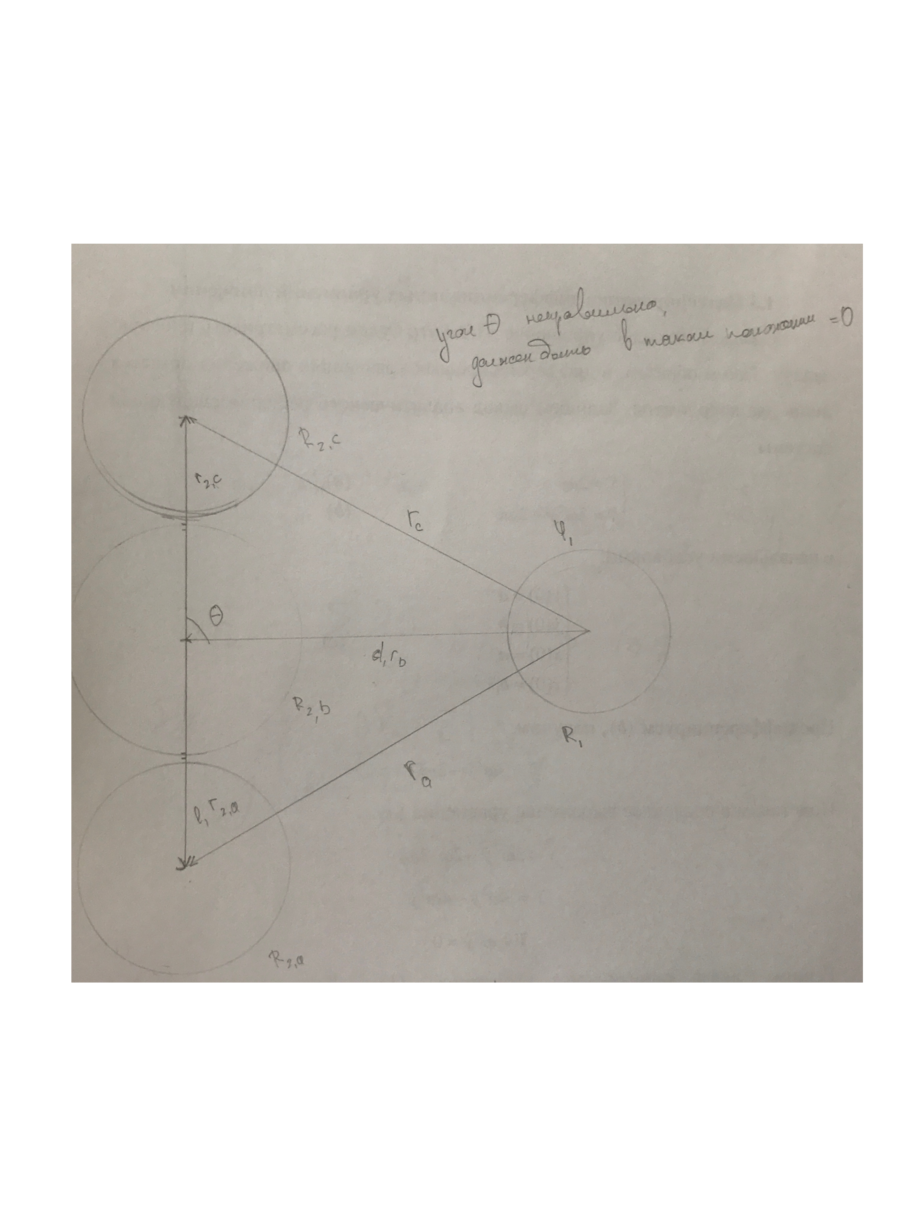
\includegraphics[scale=0.65]{3sph.png}}
	\caption{Замена космического аппарата сферами}
	\label{ris:3sph}
\end{figure}

Для моделирования взаимодействия составим обратную матрицу ёмкостей $[C_m]^{-1}$ (\ref{eq:cm_inv}):
\begin{equation}
\label{eq:3sph_cm}
	[C_m]^{-1} = 
	\begin{pmatrix}
		1/R_1	&	1/r_a	&	1/r_b	&	1/r_c\\
		1/r_a	&	1/R_{2a}	&	1/l		&	1/2l\\
		1/r_b	&	1/l		&	1/R_{2b}	&	1/l\\
		1/r_c	&	1/2l		&	1/l		&	1/R_{2c}
	\end{pmatrix},
\end{equation}
где $R_1$ – радиус внешней сферы, $R_{2a}$ – радиус сферы $A$ тела $2$, $R_{2b}$ – радиус сферы $B$ тела $2$, $R_{2c}$ – радиус сферы $C$ тела $2$, $l$ – расстояние между центрами соседних сфер (сферы $A$ и сферы $B$, сферы $B$ и сферы $C$),

\noindent $r_a = \norm{\vec{R}_a}$ – расстояние между центром внешней сферы и центром сферы $A$ тела $2$, $r_b = \norm{\vec{R}_b}$ – расстояние между центром внешней сферы и центром сферы $B$ тела $2$, $r_c = \norm{\vec{R}_c}$ – расстояние между центром внешней сферы и центром сферы $C$ тела $2$.

Для описания векторов $\vec{R_a}$, $\vec{R_b}$, $\vec{R_c}$ введем вектор $\vec{A}$  описывающий расстояния между центром тела $2$ и центром внешней сферы:
\begin{equation}
\label{eq:3sph_A}
	\vec{A} =
	\begin{pmatrix}
		0\\
		-d
	\end{pmatrix}.
\end{equation}
Так же введем вектора $\vec{L}_1$ и $\vec{L}_2$, описывающие расстояния между центрами сфер $B$ и $C$ и сфер $A$ и $B$:
\begin{equation}
\label{eq:3sph_l1}
	\vec{L}_1 = -\vec{L}_2,
\end{equation}
\begin{equation}
\label{eq:3sph_l2}
	\vec{L}_2 = 
	\begin{pmatrix}
		l \cos \theta(t)\\
		l \sin \theta(t)
	\end{pmatrix}.
\end{equation}

Имея (\ref{eq:3sph_A}), (\ref{eq:3sph_l1}) и (\ref{eq:3sph_l2}) запишем вектора $\vec{R_a}$, $\vec{R_b}$, $\vec{R_c}$:
\begin{equation}
\label{eq:3sph_Ra}
	\vec{R}_a = \vec{L}_1 - \vec{A},
\end{equation}
\begin{equation}
\label{eq:3sph_Rb}
	\vec{R}_b = -\vec{A},
\end{equation}
\begin{equation}
\label{eq:3sph_Rc}
	\vec{R}_c = \vec{L}_2 - \vec{A}.
\end{equation}

Имея (\ref{eq:3sph_Ra}), (\ref{eq:3sph_Rb}) и (\ref{eq:3sph_Rc}) можно получить обратную матрицу к матрице $[C_m]^{-1}$ (\ref{eq:3sph_cm}), тем самым решив уравнение (\ref{eq:voltage_matr}) и получив заряды сфер:
\begin{equation}
\label{eq:3sph_q_eq}
	\begin{pmatrix}
		q_1\\
		q_{2a}\\
		q_{2b}\\
		q_{2c}
	\end{pmatrix}
	= k_c C_m 
	\begin{pmatrix}
		-\phi\\
		\phi\\
		\phi\\
		\phi
	\end{pmatrix},
\end{equation}
где $q_1$ – заряд внешней сферы, $q_{2a}$ – заряд сферы $A$ тела $2$, $q_{2b}$ – заряд сферы $B$ тела $2$, $q_{2c}$ – заряд сферы $C$ тела $2$, $\phi$ – абсолютное значение напряжения для любой из сфер (оно берется одинаковым). 

Для получения зависимости угла $\theta$ от времени необходимо составить уравнение Лагранжа второго рода\cite{markeev}:
\begin{equation}
\label{eq:3sph_lag}
	\frac{d}{dt}\frac{\partial T}{\partial \dot{q_j}} - \frac{\partial T}{\partial q_j} = Q_j,
\end{equation}
где $q_j$ – обобщенные координаты, в нашем случае это $\theta(t)$, $Q_j$ – обобщенная сила,$T$ – кинетическая энергия, для нашей системы записанная в выражении:
\begin{equation}
\label{eq:3sph_kin}
	T = \frac{J \left(\frac{d \theta (t)}{dt}\right)^2}{2},
\end{equation}
где $J$ – момент инерции.

Обобщенная сила для обобщенной координаты $\theta$ имеет вид:
\begin{equation}
\label{eq:3sph_Qj}
	Q_\theta = \frac{\partial \vec{r}_{ba}}{\partial \theta(t)} \cdot F_{2a} + \frac{\partial \vec{r}_{bc}}{\partial \theta(t)} \cdot F_{2c},
\end{equation}
где вектор $\vec{r}_{ba} = L_2$ – вектор между центрами сфер $A$ и $B$, $\vec{r}_{bc} = L_1$ – вектор между центрами сфер $B$ и $C$, $F_{2a}$ и $F_{2c}$ – силы электростатического взаимодействия в центре внешней сферы:
\begin{equation}
\label{eq:3sph_F2a}
	F_{2a} = - \frac{k_c q_1 q_{2a}}{r_a^3} \vec{R}_a,
\end{equation}
\begin{equation}
\label{eq:3sph_F2c}
	F_{2c} = - \frac{k_c q_1 q_{2c}}{r_c^3} \vec{R}_c.
\end{equation}

Числено решив (\ref{eq:3sph_lag}) с учетом (\ref{eq:3sph_kin}), (\ref{eq:3sph_Qj}), (\ref{eq:3sph_F2a}) и (\ref{eq:3sph_F2c}) получим зависимость $\theta$ от времени.

Изменение угла $\theta$ для значений параметров $\phi = 20000$В, $R_1 = 0.5$м, $R_{2a} = R_{2c} = 0.59$м, $R_{2b} = 0.65$м, $l = 1.5$м, $d = 15$м, $J = 1000$кг$\cdot$м${}^2$ \cite{3sph} изображено на рисунке (\ref{ris:3sph_theta_no_fix}).
Начальные условия:
\begin{equation}
	\begin{cases}
		\theta(0) = 1,\\
		\theta'(0) = 0.
	\end{cases}
\end{equation}

Обозначим числители выражений (\ref{eq:3sph_F2a})-(\ref{eq:3sph_F2c}) $S_a = - k_c q_1 q_{2a}$ и $S_c = - k_c q_1 q_{2c}$ соответственно и назовем это перетеканием заряда (рис. \ref{ris:3sph_flow_no_fix}).

\begin{figure}[H]
	\center{\includegraphics[scale=0.7]{msm_theta_d=15_no_fix.png}}
	\caption{Зависимость угла $\theta$ от времени $t$ для заданных параметров}
	\label{ris:3sph_theta_no_fix}
\end{figure}

\begin{figure}[H]
	\center{\includegraphics[scale=0.7]{msm_flow_d=15_no_fix.png}}
	\caption{Перетекание заряда для заданных параметров}
	\label{ris:3sph_flow_no_fix}
\end{figure}

На рисунке \ref{ris:3sph_flow_no_fix} видно, что величина изменение заряда порядка $10^{-4}$.
Попробуем заменить перетекание заряда в выражениях для сил на фиксированную величину, взятую в точках пересечения $S_a$ и $S_c$, которые соответствуют $\theta = 0$.
Проведем вычисления для разных расстояний $d$.

\begin{figure}[H]
	\center{\includegraphics[scale=0.7]{msm_theta_d=20.png}}
	\caption{Зависимость угла $\theta$ от времени $t$ для $d=20$м}
	\label{ris:3sph_theta_d=20}
\end{figure}

\begin{figure}[H]
	\center{\includegraphics[scale=0.7]{msm_flow_d=20.png}}
	\caption{Перетекание заряда для $d=20$м}
	\label{ris:3sph_flow_d=20}
\end{figure}

\begin{figure}[H]
	\center{\includegraphics[scale=0.7]{msm_theta_d=15.png}}
	\caption{Зависимость угла $\theta$ от времени $t$ для $d=15$м}
	\label{ris:3sph_theta_d=15}
\end{figure}

\begin{figure}[H]
	\center{\includegraphics[scale=0.7]{msm_flow_d=15.png}}
	\caption{Перетекание заряда для $d=15$м}
	\label{ris:3sph_flow_d=15}
\end{figure}

\begin{figure}[H]
	\center{\includegraphics[scale=0.7]{msm_theta_d=10.png}}
	\caption{Зависимость угла $\theta$ от времени $t$ для $d=10$м}
	\label{ris:3sph_theta_d=10}
\end{figure}

\begin{figure}[H]
	\center{\includegraphics[scale=0.7]{msm_flow_d=10.png}}
	\caption{Перетекание заряда для $d=10$м}
	\label{ris:3sph_flow_d=10}
\end{figure}

\begin{figure}[H]
	\center{\includegraphics[scale=0.7]{msm_theta_d=5.png}}
	\caption{Зависимость угла $\theta$ от времени $t$ для $d=5$м}
	\label{ris:3sph_theta_d=5}
\end{figure}

\begin{figure}[H]
	\center{\includegraphics[scale=0.7]{msm_flow_d=5.png}}
	\caption{Перетекание заряда для $d=5$м}
	\label{ris:3sph_flow_d=5}
\end{figure}

\begin{figure}[H]
	\center{\includegraphics[scale=0.7]{{msm_theta_d=2.5}.png}}
	\caption{Зависимость угла $\theta$ от времени $t$ для $d=2.5$м}
	\label{ris:3sph_theta_d=2.5}
\end{figure}

\begin{figure}[H]
	\center{\includegraphics[scale=0.7]{{msm_flow_d=2.5}.png}}
	\caption{Перетекание заряда для $d=2.5$м}
	\label{ris:3sph_flow_d=2.5}
\end{figure}

\begin{figure}[H]
	\center{\includegraphics[scale=0.7]{{msm_theta_d=1.8}.png}}
	\caption{Зависимость угла $\theta$ от времени $t$ для $d=1.8$м}
	\label{ris:3sph_theta_d=1.8}
\end{figure}

\begin{figure}[H]
	\center{\includegraphics[scale=0.7]{{msm_flow_d=1.8}.png}}
	\caption{Перетекание заряда для $d=1.8$м}
	\label{ris:3sph_flow_d=1.8}
\end{figure}

Как видно из рисунков \ref{ris:3sph_theta_d=20} - \ref{ris:3sph_flow_d=1.8} при уменьшении расстояния $d$ фиксированное перетекание заряда (а значит и произведение зарядов) становится всё менее точным.
Отсюда можно сделать вывод, что метод многих сфер есть смысл применять при  сравнительно небольших расстояниях между объектами.